% =====================================================================
%  Relatório de resultados do survey pré-registrado — Parte 2
%  Medição e Experimentação em Engenharia de Software — 2º/2026
%  Formato ABNT (NBR 14724, 6023, 10520, 6024), mesmo padrão do protocolo.
%  Os números, quadros e figuras vêm de gerado/ (analise/relatorio.py).
%  Compilar:  ../../.venv/bin/python ../../analise/relatorio.py && tectonic relatorio.tex
% =====================================================================
\documentclass[12pt,a4paper]{article}

\usepackage[a4paper,top=3cm,left=3cm,bottom=2cm,right=2cm]{geometry}
\usepackage[brazilian]{babel}
\usepackage{fontspec}
\setmainfont{texgyretermes}[Extension=.otf,UprightFont=*-regular,BoldFont=*-bold,ItalicFont=*-italic,BoldItalicFont=*-bolditalic]
\usepackage{microtype}
\usepackage{booktabs,tabularx,array,float,longtable}
\usepackage{graphicx}
\usepackage{enumitem}
\usepackage{setspace}
\usepackage{titlesec}
\usepackage{fancyhdr}
\usepackage{amsmath}
\usepackage{caption}
\usepackage[authoryear,round]{natbib}
\setcitestyle{aysep={,},citesep={;}}
\usepackage[hidelinks]{hyperref}

\onehalfspacing
\setlength{\parindent}{1.25cm}
\setlength{\parskip}{0pt}
\emergencystretch=2em

\titleformat{\section}{\normalfont\bfseries\MakeUppercase}{\thesection}{0.6em}{}
\titlespacing*{\section}{0pt}{1.2ex}{0.6ex}
\titleformat{\subsection}{\normalfont\bfseries}{\thesubsection}{0.6em}{}
\titlespacing*{\subsection}{0pt}{1ex}{0.4ex}

\pagestyle{fancy}\fancyhf{}
\renewcommand{\headrulewidth}{0pt}
\fancyhead[R]{\thepage}
\fancypagestyle{plain}{\fancyhf{}\renewcommand{\headrulewidth}{0pt}\fancyhead[R]{\thepage}}

\addto\captionsbrazilian{\renewcommand{\tablename}{Quadro}\renewcommand{\figurename}{Figura}}
\renewcommand{\tablename}{Quadro}
\captionsetup{font=small,labelfont=bf,labelsep=endash,skip=2pt,justification=raggedright,singlelinecheck=false}
\captionsetup[table]{position=top}
\captionsetup[figure]{position=top}
\newcommand{\fonte}[1]{\par\vspace{1pt}{\footnotesize\singlespacing Fonte: #1}\par\vspace{4pt}}
\renewcommand{\arraystretch}{1.04}
\setlength{\tabcolsep}{3pt}
\setlist{nosep,leftmargin=1.2em}
\newcolumntype{L}[1]{>{\raggedright\arraybackslash}p{#1}}
\newcolumntype{Y}{>{\raggedright\arraybackslash}X}
\newcommand{\thead}[1]{\textbf{#1}}
\newcommand{\quadro}{\begin{table}[H]\centering\footnotesize\singlespacing}
\newcommand{\fimquadro}{\end{table}}

\newcommand{\nRecebidas}{56}
\newcommand{\nPreteste}{5}
\newcommand{\nOficial}{51}
\newcommand{\nDescartes}{3}
\newcommand{\nValidas}{48}
\newcommand{\nUsuarios}{46}
\newcommand{\margem}{14,1}
\newcommand{\margemU}{14,4}
\newcommand{\medianaDur}{183}
\newcommand{\limiteDur}{61}
\newcommand{\minDur}{87}
\newcommand{\primeira}{14/11/2026}
\newcommand{\ultima}{26/11/2026}
\newcommand{\alfaCON}{0,63}
\newcommand{\alfaCONlo}{0,41}
\newcommand{\alfaCONhi}{0,80}
\newcommand{\alfaPRA}{0,37}
\newcommand{\alfaPRAlo}{$-$0,14}
\newcommand{\alfaPRAhi}{0,61}
\newcommand{\nTestes}{22}
\newcommand{\pctMelhorou}{68,8}
\newcommand{\melhorouLo}{54,7}
\newcommand{\melhorouHi}{80,1}
\newcommand{\melhorouMargem}{13,1}
\newcommand{\pctPiorou}{22,9}
\newcommand{\pctUsoAlto}{93,7}
\newcommand{\medianaMtres}{4,67}
\newcommand{\pctPRAquatro}{96}
\newcommand{\pctPRAquatroTot}{74}
\newcommand{\pctCONum}{98}
\newcommand{\nABR}{15}
\newcommand{\rhoHdoisB}{0,40}
\newcommand{\pHdoisB}{0,006}
\newcommand{\pHolmHdoisB}{0,092}
\newcommand{\pOrigHdoisB}{0,035}
\newcommand{\rhoPRAdoisCONF}{0,57}
\newcommand{\rhoPRAdoisCONFlo}{0,36}
\newcommand{\rhoPRAdoisCONFhi}{0,73}
\newcommand{\pHolmPRAdoisCONF}{$<$\,0,001}
\newcommand{\deltaHquatroA}{$-$0,58}
\newcommand{\deltaHquatroAlo}{$-$0,85}
\newcommand{\deltaHquatroAhi}{$-$0,24}
\newcommand{\pHquatroA}{0,004}
\newcommand{\pHolmHquatroA}{0,072}
\newcommand{\dataExport}{27/11/2026}
\newcommand{\nDepois}{10}
\newcommand{\nNaoAtua}{7}
\newcommand{\nGerar}{3}
\newcommand{\nCodigo}{8}
\newcommand{\rMinHdoisA}{0,72}
\newcommand{\rMaxHdoisA}{0,88}
\newcommand{\rhoPRAdoisMin}{$-$0,12}
\newcommand{\rhoPRAdoisMax}{0,03}
\newcommand{\pctCodEst}{21}
\newcommand{\pctCodForm}{12}

\makeatletter\newcommand{\inserir}[1]{\@@input #1 }\makeatother

\hypersetup{pdftitle={Relatório de resultados: aprendizado de programação na era da IA generativa},
            pdfauthor={Grupo — Medição e Experimentação em ES}}

\begin{document}

\begin{center}
\singlespacing
{\bfseries APRENDIZADO DE PROGRAMAÇÃO NA ERA DA IA GENERATIVA}\\[0.3ex]
{\itshape Relatório de resultados do survey pré-registrado (Parte 2): versão parcial, com dados até \ultima}\\[0.8ex]
Ana Luiza Santos Gomes, Bruna Barbosa Portilho Bernardes, Guilherme Augustto Costa Barros e Vinícius Dias\\
{\small Pontifícia Universidade Católica de Minas Gerais (PUC Minas), Unidade Lourdes\\
Engenharia de Software · Medição e Experimentação em Engenharia de Software · 2º/2026\\
Repositório: \href{https://github.com/guicostak/Trabalho-Final-Survey}{github.com/guicostak/Trabalho-Final-Survey}}
\end{center}
\vspace{-1ex}

\section{Introdução}

Este relatório apresenta os resultados do survey cujo protocolo foi registrado em 13/11/2026 (Parte 1). Pelo modelo GQM \citep{basili}, o objetivo é \emph{analisar} o uso de IA generativa no aprendizado de programação, \emph{com o propósito de} caracterizar associações, \emph{com respeito ao} aprendizado de conceitos, à prática de escrita de código e à confiança para programar sem IA, \emph{do ponto de vista de} estudantes e profissionais formados em cursos de tecnologia, \emph{no contexto de} instituições brasileiras em 2026/2. A hipótese central, motivada por Prather et al. (2024), é que a IA favorece o entendimento de conceitos, mas pode reduzir a prática de escrita. As análises seguem o plano registrado; o que mudou está declarado na Seção~\ref{sec:desvios}. Os números vêm da exportação bruta do Microsoft Forms, processada pelo mesmo código que alimenta o dashboard (\texttt{analise/survey.py}). \textbf{Os resultados são parciais}: a coleta segue aberta até 04/12/2026 e ainda não atingiu a meta de 50 respostas válidas.

\section{Execução da coleta e qualidade dos dados}

O formulário recebeu \textbf{\nRecebidas\ respostas}. As \nPreteste\ enviadas até 13/11/2026 às 23h59, prazo da Parte 1, compõem o pré-teste e foram excluídas pela regra E0; as \nOficial\ restantes formam a coleta oficial, de \primeira\ a \ultima. Como o link é aberto, a taxa de resposta não é calculável \citep{ralph}. As regras de limpeza do protocolo, aplicadas nessa ordem e com o primeiro motivo que se aplica a cada resposta, estão no Quadro~\ref{tab:limpeza}. A mediana de duração da coleta oficial foi de \medianaDur\ s, o que fixou o limite de E4 em \limiteDur\ s; a resposta mais rápida levou \minDur\ s.

\quadro
\caption{Regras de limpeza e respostas descartadas}\label{tab:limpeza}
\begin{tabularx}{\textwidth}{@{}L{0.9cm}YL{1.6cm}L{3.2cm}@{}}
\toprule
\thead{Regra} & \thead{Motivo} & \thead{Respostas} & \thead{IDs no Forms} \\
\midrule
\inserir{gerado/tab_limpeza.tex}
\midrule
\multicolumn{2}{@{}l}{\textbf{Respostas válidas}} & \textbf{\nValidas} & Meta: 50 \\
\bottomrule
\end{tabularx}
\fonte{Dados da pesquisa, Microsoft Forms (exportação de \dataExport).}
\fimquadro

Restaram \textbf{\nValidas\ respostas válidas}, abaixo da meta de 50. A margem de erro nominal de uma proporção, com 95\% de confiança e $p = 0{,}5$, é de \textbf{$\pm$\margem\ p.p.}; por a amostra não ser probabilística, ela não garante representatividade \citep{baltes}. As questões QP2 a QP4 usam só quem usa IA, segundo o livro de códigos (frequência diferente de ``nunca'' e finalidade diferente de ``não uso IA''): \nUsuarios\ respondentes, com margem de $\pm$\margemU\ p.p. O perfil das respostas válidas está no Quadro~\ref{tab:perfil}.

\quadro
\caption{Perfil das respostas válidas}\label{tab:perfil}
\begin{tabularx}{\textwidth}{@{}L{3.2cm}Y@{}}
\toprule
\thead{Variável} & \thead{Distribuição (n e \%)} \\
\midrule
\inserir{gerado/tab_perfil.tex}
\bottomrule
\end{tabularx}
\fonte{Dados da pesquisa (2026).}
\fimquadro

A amostra concentra estudantes avançados e profissionais de ES e SI, que já atuam na área e começaram a aprender antes da popularização da IA generativa. As metas por segmento do protocolo (8 respostas por curso) não foram atingidas em CC, ADS e outros cursos, que ficam só descritivos.

\section{Confiabilidade dos construtos}

O Quadro~\ref{tab:alfa} traz o $\alpha$ de Cronbach \citep{cronbach} dos dois construtos com vários itens, nos \nUsuarios\ usuários de IA, com intervalo de confiança por bootstrap \citep{efron}.

\quadro
\caption{Confiabilidade dos construtos ($\alpha$ de Cronbach)}\label{tab:alfa}
\begin{tabularx}{\textwidth}{@{}L{3.3cm}L{0.6cm}L{0.8cm}L{2.1cm}YL{2.0cm}@{}}
\toprule
\thead{Construto} & \thead{k} & \thead{$\alpha$} & \thead{IC 95\%} & \thead{$\alpha$ sem o item} & \thead{Avaliação} \\
\midrule
\inserir{gerado/tab_alfa.tex}
\bottomrule
\end{tabularx}
\fonte{Dados da pesquisa (2026). Critério do protocolo: $\geq$ 0,70 aceitável; 0,60 a 0,70 questionável; $<$ 0,60, itens separados.}
\fimquadro

CON teve $\alpha$ = \alfaCON, valor questionável, em parte por efeito teto: \pctCONum\% concordam com CON1. PRA teve $\alpha$ = \alfaPRA, abaixo de 0,60; pela regra do protocolo, \textbf{os itens de PRA foram analisados separadamente}. A causa é PRA2 (``consigo escrever do zero, sem IA''), cuja correlação com os demais itens de PRA ficou entre \rhoPRAdoisMin\ e \rhoPRAdoisMax: ele mede a \emph{capacidade} de escrever sem IA, enquanto PRA1, PRA3 e PRA4 medem o \emph{hábito} de escrever. É uma ameaça de validade de construto, por explicação pré-operacional inadequada \citep{wohlin}.

\section{Resultados por questão de pesquisa}

O nível de significância é $\alpha = 0{,}05$, bilateral. Como PRA foi separado, cada hipótese que usava o escore M4 virou um teste por item, e a \textbf{correção de Holm} \citep{holm} foi aplicada aos \nTestes\ testes confirmatórios. Os tamanhos de efeito seguem Cohen (1988) e, para o $\delta$ de Cliff, Cliff (1993), com IC 95\% por bootstrap de 5.000 reamostragens. O Quadro~\ref{tab:hip} resume todos os testes, e o desenho transversal só permite falar em associações.

\subsection{QP1: como a IA é usada e como o seu efeito é avaliado}

Entre os \nValidas\ válidos, \pctUsoAlto\% usam IA \emph{sempre} ou \emph{frequentemente} ao estudar programação, e a finalidade mais citada é entender conceitos ou mensagens de erro (Quadro~\ref{tab:qp1}). \textbf{\pctMelhorou\% avaliam que a IA melhorou o aprendizado} (IC de Wilson de \melhorouLo\% a \melhorouHi\%; margem de $\pm$\melhorouMargem\ p.p.) \citep{wilson}, e \pctPiorou\% dizem que piorou.

\quadro
\caption{QP1: uso e avaliação da IA (respostas válidas, n = \nValidas)}\label{tab:qp1}
\begin{tabularx}{\textwidth}{@{}L{3.4cm}YL{0.6cm}L{0.9cm}L{2.4cm}L{1.4cm}@{}}
\toprule
\thead{Item} & \thead{Categoria} & \thead{n} & \thead{\%} & \thead{IC 95\% (Wilson)} & \thead{Margem} \\
\midrule
\inserir{gerado/tab_qp1.tex}
\bottomrule
\end{tabularx}
\fonte{Dados da pesquisa (2026). Categorias sem respostas foram omitidas.}
\fimquadro

A Figura~\ref{fig:likert} mostra os itens Likert em barras divergentes. A concordância com os itens de conceitos é quase unânime, enquanto os itens de prática se concentram na discordância; em PRA4, \pctPRAquatro\% concordam que, desde que passaram a usar IA, escrevem menos código por conta própria (\pctPRAquatroTot\% concordam totalmente).

\begin{figure}[H]
\centering
\caption{Itens Likert de conceitos (CON) e de prática de escrita (PRA), usuários de IA (n = \nUsuarios)}\label{fig:likert}
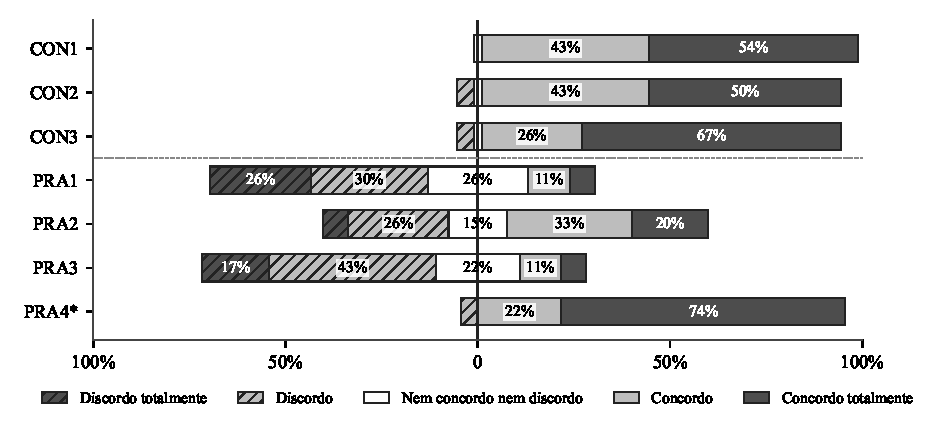
\includegraphics[width=\textwidth]{gerado/fig_likert.pdf}
\fonte{Dados da pesquisa (2026). *PRA4 é mostrado como respondido; na análise, é invertido (6 $-$ x).}
\end{figure}

\subsection{QP2: a IA favorece conceitos em detrimento da prática de escrita?}

\textbf{H2a foi confirmada nos quatro itens}: o escore de conceitos (mediana de \medianaMtres) supera cada item de prática, com efeitos grandes ($r$ de \rMinHdoisA\ a \rMaxHdoisA; $p_{\text{Holm}} < 0{,}001$; Figura~\ref{fig:h2a}). Como CON e PRA são itens diferentes, o resultado indica um padrão relativo, não uma diferença na mesma régua. A frequência de uso se associou positivamente ao aprendizado de conceitos (H2b: $\rho$ = \rhoHdoisB; $p$ = \pHdoisB), mas a associação não resistiu à correção ($p_{\text{Holm}}$ = \pHolmHdoisB). As correlações entre uso e prática (H2c) foram negativas em três dos quatro itens, todas sem significância.

\begin{figure}[H]
\centering
\caption{H2a: escore de conceitos (M3) e itens de prática de escrita, usuários de IA (n = \nUsuarios)}\label{fig:h2a}
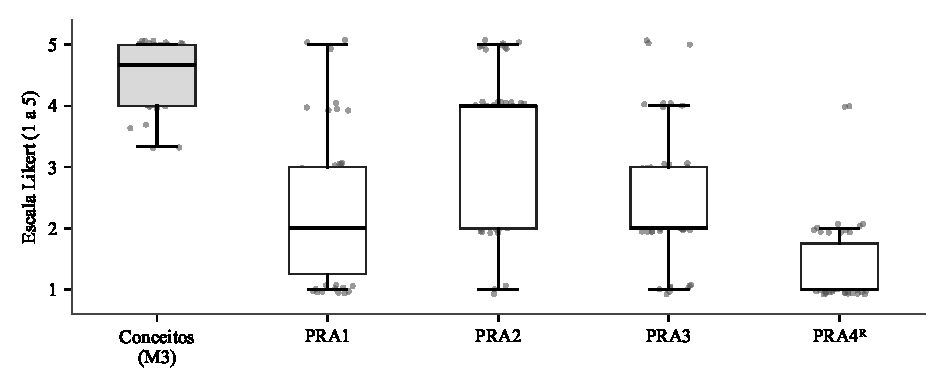
\includegraphics[width=\textwidth]{gerado/fig_h2a.pdf}
\fonte{Dados da pesquisa (2026). Caixas: mediana e intervalo interquartil; pontos: respondentes (com dispersão para visualização).}
\end{figure}

\subsection{QP3: finalidade, prática e confiança para programar sem IA}

Na comparação por finalidade (H3a), ``gerar exemplos ou exercícios'' teve n = \nGerar, e a regra condicional (i) agrupou as finalidades em ``código pronto'' (n = \nCodigo) e ``demais''. Quem busca código pronto relatou menos prática nos quatro itens ($\delta < 0$), mas sem significância. Em H3b, \textbf{só PRA2 se associou à confiança}, com efeito grande ($\rho$ = \rhoPRAdoisCONF; IC de \rhoPRAdoisCONFlo\ a \rhoPRAdoisCONFhi; $p_{\text{Holm}}$ \pHolmPRAdoisCONF). Os itens de hábito não se associaram à confiança. Como PRA2 e CONF têm conteúdo próximo, parte dessa correlação pode ser sobreposição de construtos.

\subsection{QP4: quem começou depois da IA pratica menos?}

Em H4a, quem começou a aprender a partir de 2023 (n = \nDepois) relatou menor capacidade de escrever do zero (PRA2: $\delta$ = \deltaHquatroA; IC de \deltaHquatroAlo\ a \deltaHquatroAhi; $p$ = \pHquatroA), mas o resultado não resistiu a Holm ($p_{\text{Holm}}$ = \pHolmHquatroA) e fica como hipótese para estudos futuros. H4b ficou só descritiva, porque quem não atua na área somou n = \nNaoAtua\ (regra iii). Em H4c, com SIT e IAU agrupadas (regra ii), \pctCodEst\% dos estudantes e \pctCodForm\% dos formados buscam código pronto, diferença não significativa pelo teste exato de Fisher.

{\footnotesize\singlespacing
\begin{longtable}{@{}L{1.8cm}L{2.2cm}L{0.6cm}L{1.15cm}L{1.15cm}L{3.85cm}L{1.7cm}L{1.6cm}@{}}
\caption{Testes confirmatórios (usuários de IA, n = \nUsuarios; Holm sobre \nTestes\ testes)}\label{tab:hip}\\
\toprule \thead{Hipótese} & \thead{Teste} & \thead{n} & \thead{$p$} & \thead{$p$ Holm} & \thead{Efeito [IC 95\%]} & \thead{Magnitude} & \thead{Decisão} \\ \midrule \endfirsthead
\toprule \thead{Hipótese} & \thead{Teste} & \thead{n} & \thead{$p$} & \thead{$p$ Holm} & \thead{Efeito [IC 95\%]} & \thead{Magnitude} & \thead{Decisão} \\ \midrule \endhead
\inserir{gerado/tab_hipoteses.tex}
\bottomrule
\multicolumn{8}{@{}L{15.9cm}@{}}{\scriptsize Regras condicionais do protocolo: (i) finalidade com n $<$ 5, comparação ``código pronto'' $\times$ ``demais''; (ii) SIT e IAU em duas categorias; (iii) grupo com n $<$ 10, só descritiva (fora de Holm). $\delta$ = $\delta$ de Cliff. Os IC do $r$ de Wilcoxon ficam estreitos porque quase todas as diferenças têm o mesmo sinal.}
\end{longtable}
\vspace{-6pt}\fonte{Dados da pesquisa (2026).}
}

\subsection{Análise de sensibilidade}

Para mostrar quanto as decisões dependem da separação dos itens, as hipóteses foram refeitas com o escore M4 e a família original de testes (Quadro~\ref{tab:sens}). H2a continua significativa, e \textbf{H2b também passa} ($p_{\text{Holm}}$ = \pOrigHdoisB); as demais, não. A conclusão central (QP2) não depende da regra de separação; a de H2b, sim.

\quadro
\caption{Sensibilidade: plano original, com M4 como escore único}\label{tab:sens}
\begin{tabularx}{\textwidth}{@{}L{2.4cm}YL{1.6cm}L{3.2cm}L{2.2cm}@{}}
\toprule
\thead{Hipótese} & \thead{Efeito} & \thead{$p$} & \thead{$p$ Holm (plano original)} & \thead{Decisão} \\
\midrule
\inserir{gerado/tab_sensibilidade.tex}
\bottomrule
\end{tabularx}
\fonte{Dados da pesquisa (2026). H4b ficou só descritiva também nesse cenário (regra iii).}
\fimquadro

\section{Resposta aberta}

Houve \nABR\ respostas abertas válidas. A análise temática indutiva \citep{braun} gerou cinco temas provisórios: risco à prática e aos fundamentos; a IA facilita entender conceitos e erros; o efeito depende do modo de uso e da base prévia; mudança do papel do programador, de digitar para projetar e revisar; e pressão por produtividade e dependência. Os temas repetem o achado quantitativo: a IA ajuda a entender, mas pode tirar a prática, sobretudo de quem está começando. A dupla codificação com $\kappa$ de Cohen, prevista no protocolo, ainda está pendente, e os temas devem ser lidos como provisórios.

\section{Desvios em relação ao protocolo}\label{sec:desvios}

Os desvios estão detalhados em \texttt{DESVIOS.md} e na página de metodologia do dashboard, e foram declarados conforme os Registered Reports \citep{ralph}. Em resumo: (D1) o pré-teste teve 5 respostas, não 4, e elas foram filtradas pela regra E0, não apagadas; (D2) a coleta começou antes do previsto, com 2 respostas em 14/11, e se concentrou em 25 e 26/11; (D3) a análise usa um corte parcial, com \nValidas\ válidas, e a coleta segue até 04/12, com extensão possível até 11/12; (D4) PRA teve $\alpha < 0{,}60$, e a família de Holm passou de 7 para \nTestes\ testes; (D5) as regras condicionais (i), (ii) e (iii) foram aplicadas; (D6) as metas por segmento não foram atingidas em CC e ADS; (D7) a dupla codificação da resposta aberta está pendente; e (D8) a mediana de E4 foi calculada sobre a coleta oficial.

\section{Ameaças à validade e limitações}

\textbf{Conclusão:} com n = \nUsuarios, o estudo só detecta efeitos grandes, e a família de \nTestes\ testes torna a correção mais rígida; resultados não significativos não indicam ausência de efeito. \textbf{Construto:} PRA mistura capacidade e hábito, CON tem efeito teto, e admitir dependência de IA está sujeito a desejabilidade social. \textbf{Interna:} o desenho é transversal e não permite afirmar que a IA \emph{causa} menos prática; o momento de início do aprendizado (MOM) se confunde com o tempo de experiência. \textbf{Externa:} a amostra é não probabilística, concentrada em ES e SI, em quem já atua e na rede do grupo, e coletada em cerca de 26 horas; os resultados valem para esse perfil, no segundo semestre de 2026.

\section{Conclusão}

Com os dados parciais, a hipótese central foi confirmada: os respondentes \textbf{reconhecem que a IA ajuda a entender conceitos e, ao mesmo tempo, relatam pouca prática de escrita de código sem IA}, com efeito grande e robusto à forma de análise. A confiança para programar sem IA acompanha a \emph{capacidade} declarada de escrever do zero, e não o \emph{hábito} de praticar. O indício de que quem começou a aprender depois da IA escreve com menos autonomia não resistiu à correção e merece um estudo com mais iniciantes. Numa próxima rodada, PRA deve ser dividido em dois construtos (capacidade e hábito), com pelo menos três itens cada.

\begingroup
\singlespacing
\renewcommand{\refname}{Referências}
\raggedright
\setlength{\parindent}{0pt}
\begin{thebibliography}{99}\setlength{\itemsep}{3pt}\setlength{\parskip}{0pt}
\bibitem[BALTES; RALPH(2022)]{baltes} BALTES, S.; RALPH, P. Sampling in software engineering research: a critical review and guidelines. \emph{Empirical Software Engineering}, v. 27, n. 4, art. 94, 2022. DOI: 10.1007/s10664-021-10072-8.
\bibitem[BASILI; CALDIERA; ROMBACH(1994)]{basili} BASILI, V. R.; CALDIERA, G.; ROMBACH, H. D. The goal question metric approach. In: \emph{Encyclopedia of Software Engineering}. New York: Wiley, 1994.
\bibitem[BRAUN; CLARKE(2006)]{braun} BRAUN, V.; CLARKE, V. Using thematic analysis in psychology. \emph{Qualitative Research in Psychology}, v. 3, n. 2, p. 77--101, 2006.
\bibitem[CLIFF(1993)]{cliff} CLIFF, N. Dominance statistics: ordinal analyses to answer ordinal questions. \emph{Psychological Bulletin}, v. 114, n. 3, p. 494--509, 1993.
\bibitem[COHEN(1988)]{cohen} COHEN, J. \emph{Statistical power analysis for the behavioral sciences}. 2. ed. Hillsdale: Lawrence Erlbaum, 1988.
\bibitem[CRONBACH(1951)]{cronbach} CRONBACH, L. J. Coefficient alpha and the internal structure of tests. \emph{Psychometrika}, v. 16, n. 3, p. 297--334, 1951.
\bibitem[EFRON; TIBSHIRANI(1993)]{efron} EFRON, B.; TIBSHIRANI, R. J. \emph{An introduction to the bootstrap}. New York: Chapman \& Hall, 1993.
\bibitem[HOLM(1979)]{holm} HOLM, S. A simple sequentially rejective multiple test procedure. \emph{Scandinavian Journal of Statistics}, v. 6, n. 2, p. 65--70, 1979.
\bibitem[PRATHER et al.(2024)]{prather} PRATHER, J. et al. The widening gap: the benefits and harms of generative AI for novice programmers. In: ICER, 2024, Melbourne. \emph{Proceedings} [...]. New York: ACM, 2024. DOI: 10.1145/3632620.3671116.
\bibitem[RALPH et al.(2021)]{ralph} RALPH, P. et al. \emph{ACM SIGSOFT Empirical Standards}: Questionnaire Surveys; Registered Reports. 2021. Disponível em: https://github.com/acmsigsoft/EmpiricalStandards. Acesso em: 27 nov. 2026.
\bibitem[WILSON(1927)]{wilson} WILSON, E. B. Probable inference, the law of succession, and statistical inference. \emph{Journal of the American Statistical Association}, v. 22, n. 158, p. 209--212, 1927.
\bibitem[WOHLIN et al.(2012)]{wohlin} WOHLIN, C. et al. \emph{Experimentation in Software Engineering}. Berlin: Springer, 2012.
\end{thebibliography}
\endgroup

\end{document}
